\documentclass{article}
\usepackage[margin=1in]{geometry}
\usepackage{graphicx}
\usepackage{xcolor}
\usepackage{float}
\usepackage{amsmath}
\usepackage{cite}
\usepackage{hyperref}
\usepackage{indentfirst}
\graphicspath{{..} {./images}}

\definecolor{navy-blue}{rgb}{0.22,0.38,0.71}

\renewcommand{\contentsname}{\vspace*{-2\baselineskip}}

\hypersetup{
	colorlinks,
	linkcolor=black,
	urlcolor=blue,
	citecolor=black
}
  		
\begin{document}
\begin{titlepage}
	\centering
	{\huge Lab 7 - Digital Modulation: Frame Synchronization}\\[0.25 in]
	
\includegraphics[width=0.6\textwidth]{ua_logo.png}\\[0.25 in]
	{\large \textbf{ECE 531 - Software Defined Radio\\[0.25 in]
	April 18, 2025\\[0.25 in]}}
	{\large Owen Sowatzke, osowatzke@arizona.edu\\[0.05 in]
	Department of Electrical \& Computer Engineering\\[0.05 in]
	University of Arizona, Tucson, AZ 85721\\[0.5 in]}
	\hypersetup{linkcolor=navy-blue}
	\noindent\hrulefill
	\tableofcontents
	\noindent\hrulefill
\end{titlepage}

% \setlength{\parindent}{0pt}

\section{Introduction}
%Introduction to the laboratory experiment, including a brief description of the objectives and goals.

In this lab, we perform frame synchronization on data generated in MATLAB. Correct frame alignment is critical for correctly recovering the transmitted data. To detect the start of a packet, we specifically cross-correlate our received data with a known preamble. As part of our work in this lab, we learn how to perform cross-correlation with MATLAB's \texttt{filter} command. We also explore performance tradeoffs between the \texttt{xcorr} and \texttt{filter} commands. Finally, we implement a custom frame synchronization routine and evaluate its detection probabilities and packet error rates. The work that follows is divided into two sections. One provides the procedures for each of our experiments, and the other presents the results.

\section{Procedure}
% Detailed explanation of the laboratory experiment, including the design, implementation, and testing of the system.

In this section, we provide the procedure for each of our experiments. We perform frame synchronization (i.e. detect the start of frames) that are consistent with the structure shown Figure \ref{fig::frame_structure}.

\begin{figure}[H]
	\centerline{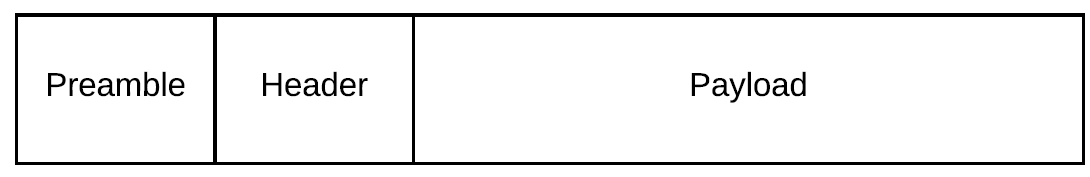
\includegraphics[width=0.6\textwidth]{frame_structure.png}}
	\caption{Frame Structure of Wireless Packet.}
	\label{fig::frame_structure}
\end{figure}

\noindent The preamble in our frames is known by both the transmitter and receiver. For our experiments, we specifically use concatenated barker sequences. Because the preamble is known by both the transmitter, we can cross-correlate our received data with the preamble using the following equation:

\begin{equation}
	C_{xy}(k) = \sum_{m}{x^*(m)y_n(m+k)}
\end{equation}

\noindent Then, we can use the peak of the cross-correlation output to determine the delay of the frame. In the lab, we execute the provided \texttt{lab7part1.m} script to perform frame synchronization. This script uses MATLAB's \texttt{xcorr} command to perform the cross-correlation. The \texttt{xcorr} command produces an output that is $2L_r - 1$ samples long, where $L_r$ is the length of the longest sequence. The center of its output corresponds to zero delay. Therefore, we can estimate the delay of our frame ($\hat{p}$) as follows:

\begin{equation}
	\hat{p} = \underset{k}{\text{argmax}}\ C_{ra}(k) - L_r
\end{equation}

\noindent For our first experiment, we replace the \texttt{xcorr} command in \texttt{lab7part1.m} with the \texttt{filter} command. Then, we validate the correctness of our implementation and compare its execution time to the original execution time for different preamble lengths. Next, we use the template given in \texttt{lab7part2.m} and the example given in \texttt{lab7part1.m} to implement a custom frame synchronization routine. Finally, we evaluate the performance of our custom frame synchronization routine across SNRs in range [0,10] dB. As part of our performance analysis, we generate plots of the detection probability and packet error rate.
 
\section{Results}
% Results and discussion of the laboratory experiment, including captured outputs, observations, and responses to laboratory questions.

In this section, we provide the results for each of our experiments. In our experiments, we specifically implement cross-correlation with MATLAB's \texttt{filter} function and compare its execution time to the \texttt{xcorr} command. Then, we create a custom frame synchronization routine and evaluate its detection probabilities and packet error rates for different SNRs.

In Figure \ref{fig::xcorr_preamble_detect}, we show the cross-correlation outputs generated by \texttt{lab7part1.m}, which uses MATLAB's \texttt{xcorr} command to perform the correlation. Note that our cross-correlation output includes a large zero regions. This region exists because we are zero-padding our sequence and time-advancing it for each point left of the midpoint. This results in element-wise multiplication with zeros, which results in a zero sum.

\begin{figure}[H]
	\centerline{\fbox{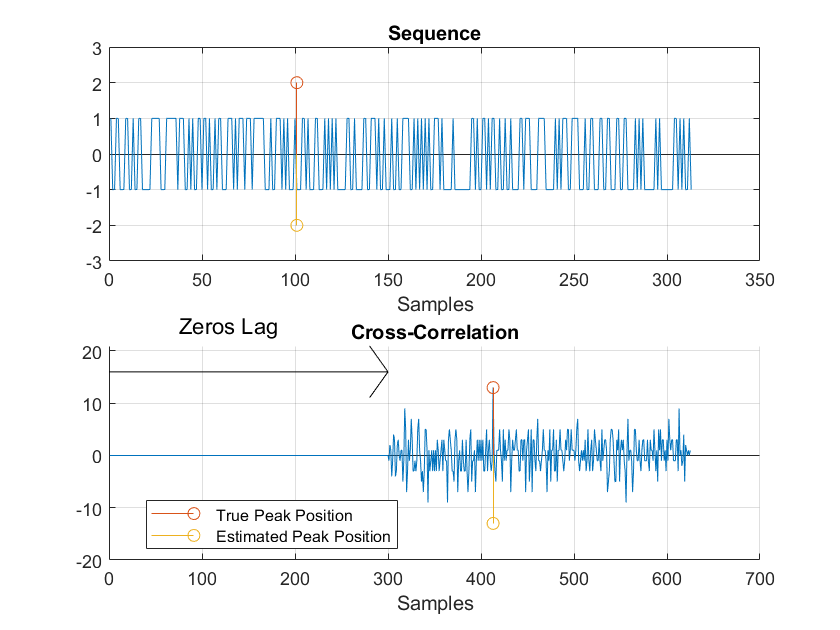
\includegraphics[width=0.5\textwidth]{xcorr_preamble_detect.png}}}
	\caption{Detecting Start of Preamble with \texttt{xcorr} Command}
	\label{fig::xcorr_preamble_detect}
\end{figure}

The \texttt{xcorr} function uses an FFT to perform a correlation, which can be slow for short sequences. As a result, we replace the \texttt{xcorr} function with a \texttt{filter} function. The filter function implements convolution of the following form:

\begin{equation}
	z(k) = \sum_{k}{y(k)h(n-k)}
\end{equation}

\noindent We can perform cross-correlation with convolution by letting $h(k) = x^*(-k)$. In other words, we can use a flipped and conjugated version of our preamble as a matched filter. Doing so, we get the results shown in Figure \ref{fig::filter_preamble_detect}.

\begin{figure}[H]
	\centerline{\fbox{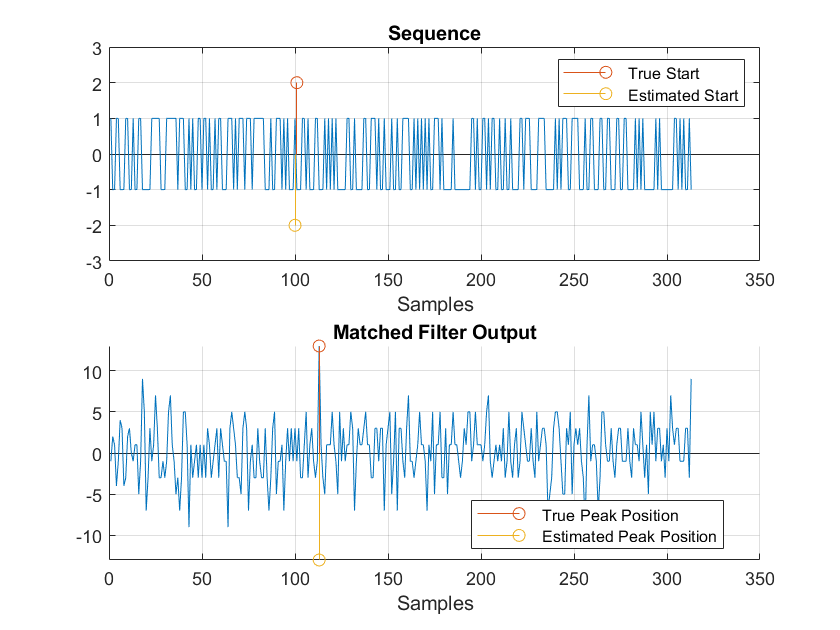
\includegraphics[width=0.5\textwidth]{filter_preamble_detect.png}}}
	\caption{Detecting Start of Preamble with \texttt{filter} Command}
	\label{fig::filter_preamble_detect}
\end{figure}

\noindent Note that the peak from our \texttt{filter} output occurs in a different location. However, we get the same delay estimate as the \texttt{xcorr} function if we account for the offsets in our output. The filter output specifically peaks when the last sample of our preamble is input to the filter. If our preamble length is given by $L_p$, we can estimate the delay from our filter output $z(k)$ as follows:

\begin{equation}
	\hat{p} = \underset{k}{\text{argmax}}\ z(k) - L_p
\end{equation}

\noindent In Figure \ref{fig::execution_time}, we compare the execution time of the \texttt{xcorr} and \texttt{filter} commands for sequence lengths in range [10, 2000]. For each sequence length, we perform also perform 1000 Monte Carlo runs to estimate the average runtime.
 
\begin{figure}[H]
	\centerline{\fbox{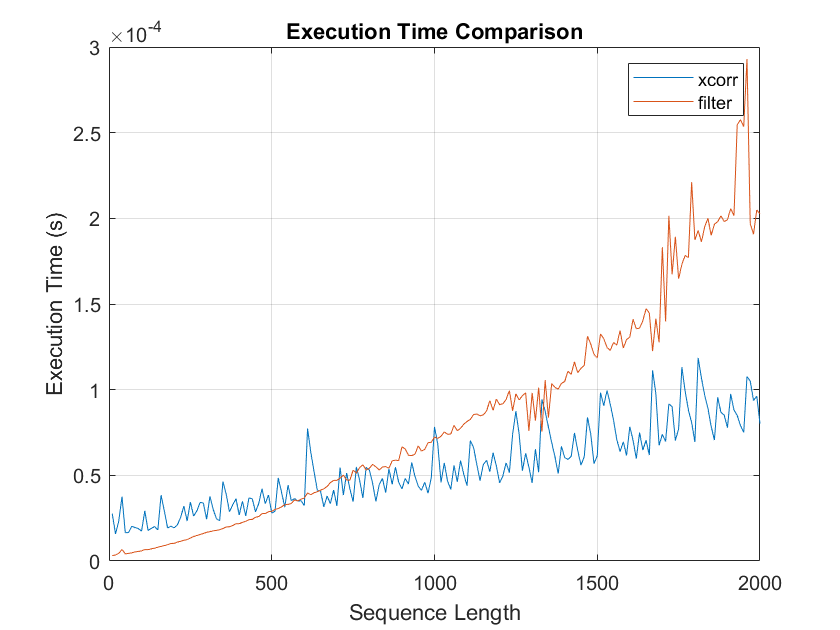
\includegraphics[width=0.5\textwidth]{execution_time.png}}}
	\caption{Comparison of \texttt{xcorr} and \texttt{filter} Execution Time}
	\label{fig::execution_time}
\end{figure}

\noindent Examining the execution times of both routines, we see that the \texttt{filter} command is faster for small sequence lengths ($< 500$), while the \texttt{xcorr} routine is faster for large filter lengths ($> 500$). For small filter lengths, time-domain filtering ( i.e. \texttt{filter}) is faster than frequency-domain filtering (i.e. \texttt{xcorr}) because it avoids the overhead of doing FFTs/IFFTs. However, as the filter length increases, the complexity increases faster for time-domain filters than it does for frequency-domain filters. In Figure \ref{fig::speedup}, we compute the speedup of the \texttt{filter} routine by dividing the average execution time of the \texttt{filter} command by the average execution time of the \texttt{xcorr} command. Examining the figure, we see that the \texttt{filter} command is approximately 8x faster for sequence lengths of 10, but is roughly half as fast for sequence lengths of 2000. The sequence lengths we use for the rest of the lab are small ($<< 500$), so we use the \texttt{filter} command.  

\begin{figure}[H]
	\centerline{\fbox{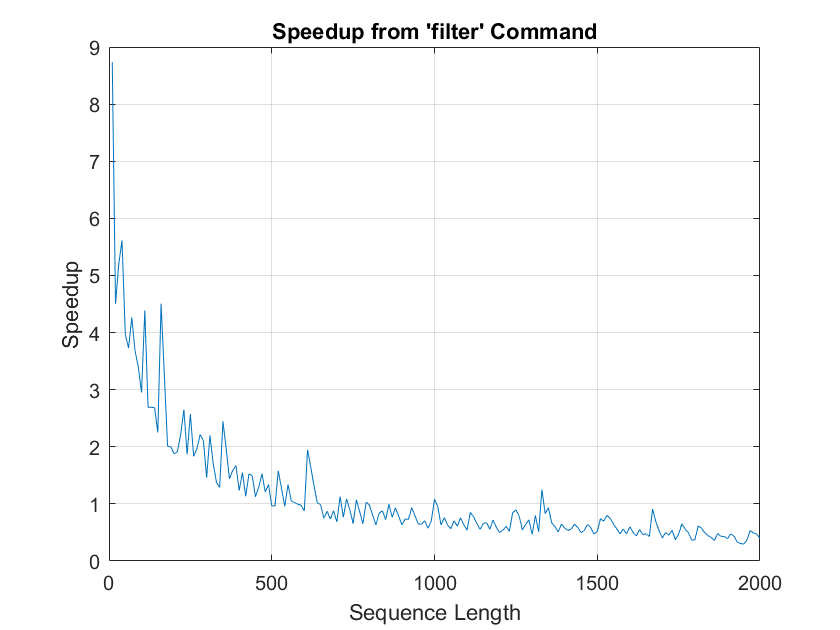
\includegraphics[width=0.5\textwidth]{speedup.png}}}
	\caption{Speedup from \texttt{filter} Command}
	\label{fig::speedup}
\end{figure}

Next, we implement a custom frame synchronizer in MATLAB. Our frame synchronizer uses the \texttt{filter} command to cross-correlate the received data with then preamble. It then normalizes the cross-correlation output to a range between 0 and 1 using the following formula:

\begin{equation}
	r(k) = \frac{C_{xy}(k)}{\sqrt{\sum_m{|x(m)|^2}}\sqrt{\sum_m{|y(m)|^2}}}
\end{equation}

\noindent This formula closely resembles the normalized correlation coefficient, which is described in \cite{pearson_correlation_coefficient}. The normalization function scales the input data, so it has a unit average power and divides the resulting correlation output by the code length. This makes the peak of the correlation output 1 instead of the preamble length. Whenever the magnitude of the normalized correlation output exceeds a threshold ($|r(k)| > T$), we mark the sample as the start of a preamble. For a more efficient hardware implementation, we can also implement the comparison as follows:

\begin{equation}
	|C_{xy}(k)|^2 > T^2\left(\sum_m{|x(m)|^2}\right)\left(\sum_m{|y(m)|^2}\right) = \alpha\sum_m{|x(m)|^2}
\end{equation}

\noindent Using our custom routine, we generate a receiver operating characteristics (ROC) curve, which is included in Figure \ref{}.

 


\noindent We assume that the input and sequence are zero mean (a valid assumption). Additionally, we can pre-compute the correlation of the preamble to reduce the amount of real-time computation. To determine detections, we compare the absolution value of the correlation $|r|$ to a threshold $T$. Simplifying, we obtain:

\begin{equation}
	\left[\sum_{i=1}^n{x_i}{y_i}\right]^2
\end{equation}



\section{Conclusion}
% Conclusions to the overall lab that discuss meaningful lessons learned and other takeaways from the assignment. (Important)

\bibliographystyle{IEEEtran}
\bibliography{sources}{}

\end{document}